\chapter{cgDNA$+$ model} \label{c2}
% https://casegroup.rutgers.edu/lnotes/dnab.pdf
% DNA mechanics plays a crucial role in several biological processes, such as nucleosome positioning~\cite{segal2009controls,segal2006genomic}, indirect readout~\cite{chen2001indirect,napoli2006indirect}, and DNA looping~\cite{schleif1992dna}.
% Along with the base composition of the dimer-step, non-local sequence contexts are also important in its mechanics~\cite{mack2001intrinsic,yanagi1991analysis,pasi2014muabc,lankavs2003dna,dixit2005molecular,young2022revisiting}.
% Notably, sequence-dependent mechanics of DNA is often considered as the \say{secondary genetic code} owing to its quintessential role in DNA readout.
% Such direct evidence piqued significant interest in understanding the sequence-dependent mechanics of DNA.
% However, the immense sequence space of DNA makes it impossible to investigate all sequences (even for DNA dodecamers) either experimentally or using atomistic molecular dynamics simulations.
% An excellent alternative is coarse-grained models that implicitly treat unessential degrees of freedom, thus allowing efficient sampling for longer simulation times or directly predicting equilibrium probability distributions. 

% With computational efficiency in mind, several coarse-grained models~\cite{xraydata,3spn,oxdna2,dnamartini,ouldridge2011structural} have been developed to better understand the role of DNA in biology. 
%However, most coarse-grained models do not capture an accurate sequence-dependent mechanical behavior of DNA due to either the model's objective or modeling assumptions.
% For instance, using dimer-dependent parameters, base-pair models can not capture non-local sequence dependence~\cite{xraydata} or the oxDNA model~\cite{ouldridge2011structural,oxdna2} focuses primarily on the thermodynamics of DNA.
% The Maddocks group introduces a novel rigid base coarse-grained model of DNA, cgDNA~\cite{cgDNA1,petkevivciute2014cgdna} trained on state-of-the-art atomistic MD simulations that accurately captures the non-local sequence-dependent mechanics of B-DNA.
%Given a parameter set, the cgDNA model predicts the probability distribution function for an arbitrary DNA sequence (in standard A, T, C, and G alphabets).
%The novelty in the cgDNA model lies in the fact that individual base-pair steps cannot achieve their local minima simultaneously, and frustration of energy surfaces arises in the nearest neighbors; thus, it naturally captures the non-local sequence-dependence in the DNA mechanics but only using dimer dependent parameters.
%This chapter introduces an extension of the cgDNA model, the cgDNA$+$ model~\cite{patelithesis} which explicitly treats base and phosphate as rigid units.

The central theme of this chapter is to provide an overview of the cgDNA$+$ model and its training~\cite{patelithesis}.
First, we have discussed the coarse-graining of DNA atomistic configuration by fitting frames in phosphate and base units and then defining internal coordinates used in the cgDNA$+$ model.
The next part introduces the cgDNA$+$ model, the underlying assumptions, and mathematical details of how the model reconstructs groundstate and stiffness matrix given a parameter set and a sequence. 
The subsequent section describes the cgDNA$+$ model training from atomistic molecular dynamics (MD) times-series of a set of sequences.
After model description and training, this chapter discusses methods to assess the model performance and quantify various approximation errors in the model.
The last part of the chapter is a brief discussion on the cgDNA$+$ Monte Carlo code~\cite{cgdnamc}, which allows efficient sampling of cgDNA$+$ predicted Gaussian probability density function (pdf) and thus, computing the expectation of any interesting physical observables for an ensemble of configurations.
%%%%%%%%%%%%%%%%%%%%%%%%%%%%%%%%%%%%%%%%%%%%%%%%%%%%%%%%%%%%%%%%
%%%%%%%%%%%%%%%%%%%%%%%%%%%%%%%%%%%%%%%%%%%%%%%%%%%%%%%%%%%%%%%%
%%%%%%%%%%%%%%%%%%%%%%%%%%%%%%%%%%%%%%%%%%%%%%%%%%%%%%%%%%%%%%%%
%%%%%%%%%%%%%%%%%%%%%%%%%%%%%%%%%%%%%%%%%%%%%%%%%%%%%%%%%%%%%%%%
%%%%%%%%%%%%%%%%%%%%%%%%%%%%%%%%%%%%%%%%%%%%%%%%%%%%%%%%%%%%%%%%
%%%%%%%%%%%%%%%%%%%%%%%%%%%%%%%%%%%%%%%%%%%%%%%%%%%%%%%%%%%%%%%%
\section{Coarse-graining of atomistic structure of dsDNA}\label{c2:sec1}
\begin{figure}[htb]
	\begin{center}
	\centering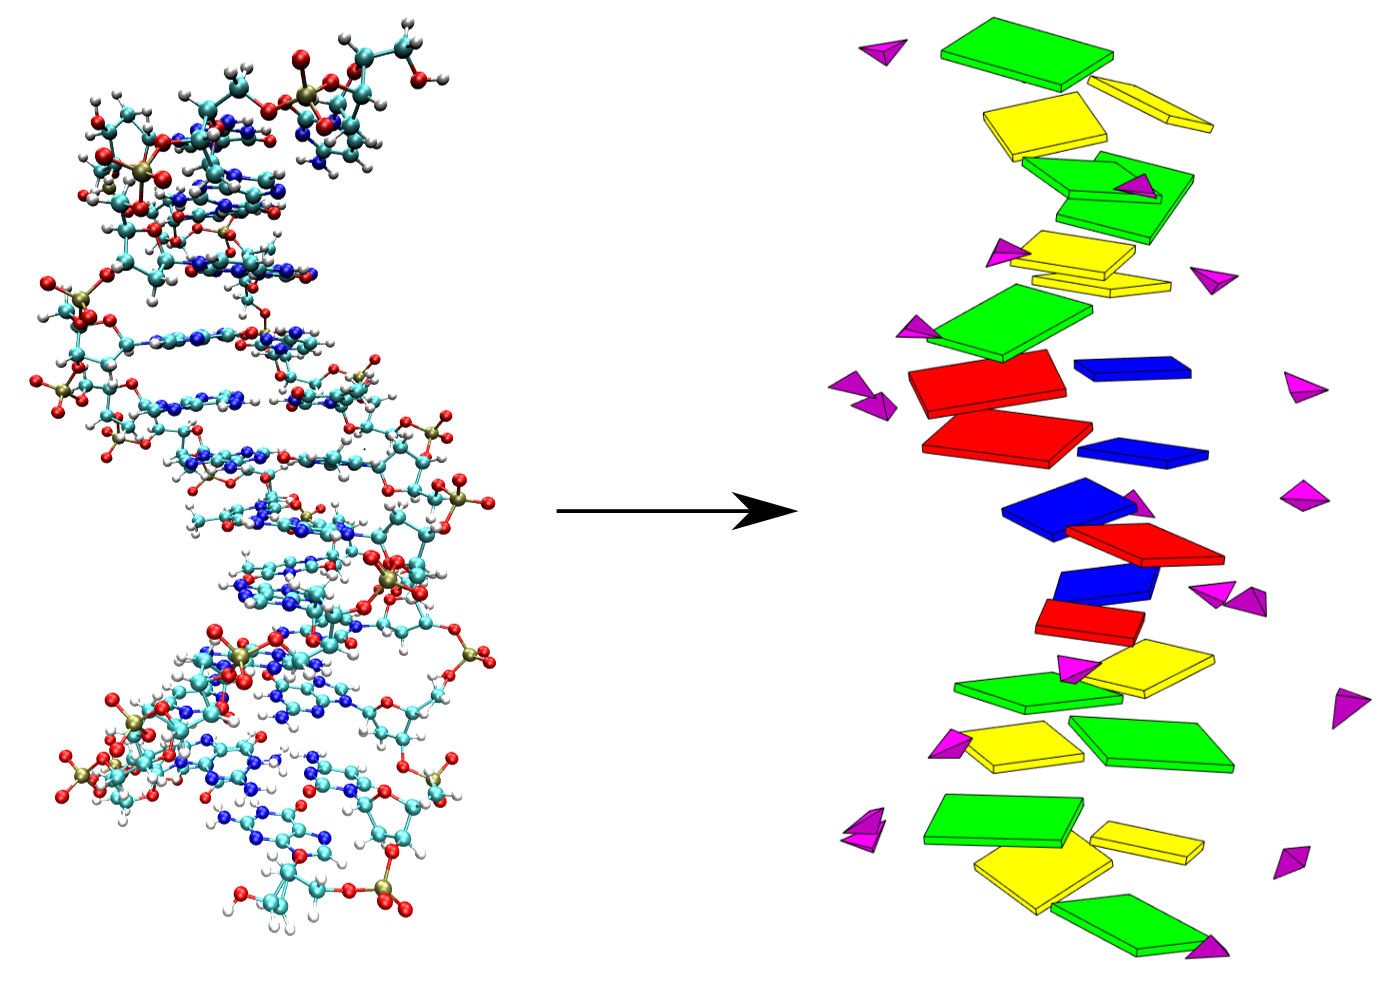
\includegraphics[scale=0.2]{images/drew_atom.png}
	\centering\caption{Coarse-graining of atomistic structure of DNA oligomer to cgDNA$+$ cartoon representation by embedding frames in bases and phosphates. }
\label{c2:fig1}
\end{center}
\end{figure}
\begin{table}
\begin{tabular}{ m{0.2cm} | m{6.4cm} | m{6.8cm} }
1  & Compute weighted centroids & $\bar{\v x} = \dfrac{\sum_{i=1}^{n}w_i \v x_i }{\sum_{i=1}^{n} w_i }$ \&  $\bar{\v y} = \dfrac{\sum_{i=1}^{n}w_i \v y_i }{\sum_{i=1}^{n} w_i }$  \\ [0.7cm]
2 & Compute centred vectors     & $\v p_i := \v x_i - \bar{\v x}$ \&   $\v q_i := \v y_i - \bar{\v y}$ \\  [0.5cm]
3 & Compute covariance matrix & $\R^{3 \times 3} \ni S = PWQ$ where $P,Q \in \R^{3 \times n}$  \linebreak with $p_i,q_i$ as their columns, respectively \linebreak and $W =  diag(w_1,w_2,...,w_n)$  \\
[0.8cm]
4 & Compute singular value decomposition & $S = U\Sigma V^T$\\ [0.2cm]
5 & Compute $R, \v r $ &
 $R = V\begin{bmatrix}
   1 &  & \\
   & 1 &  \\
    & & |VU^T|
        \end{bmatrix} U^T, \;\;\v r = \bar{\v y} - R \bar{\v x}$\\[.7cm]
\end{tabular}
\centering\caption{Algorithm to find a rigid body transformation (translation $r$ and rotation $R$) that best aligns two rigid bodies $X(x_1,x_2,...,x_n)$ and $Y(y_1,y_2,...,y_n)$ in terms of least-squares error, where $W (w_1,w_2,...,w_n)$ is the weight matrix.
This algorithm is used to fit frames in bases and phosphates.}
\label{c2:tab1}
\end{table}

This section describes the methodology to coarse-grain the atomistic representation of DNA observed in MD simulations by fitting frames in bases and phosphates.
A typical atomistic structure of dsDNA (shown in \cref{c2:fig1}) is an anti-parallel double-stranded helix whose primary structure is defined as the list of nucleotides denoted by the base name along a chosen strand from $5^\prime-$ to $3^\prime-$ direction. 
One strand is chosen as a reading strand or Watson strand, and the other is a complementary strand or Crick strand.
Using this notion, we can write the sequence of a DNA oligomer comprising of $N$ base-pair as $\sq = X_1X_2X_3...X_{N-1}X_N$ where $X_i \in$ \{A, T, C, G\}.
The complementary base of $X_i$ on the Crick strand is written as $\bar{X}_i$. 
Following the notation, $\bar{\sq}$, is written as $\bar{X}_N\bar{X}_{N-1}\bar{X}_{N-2}...\bar{X}_2\bar{X}_1$ in $5^\prime$ to $3^\prime$ direction on the Crick strand. 

The cgDNA$+$ model explicitly treats phosphates and bases as rigid units and fits $SE(3)$ frame (see appendix \cref{a3:s3}) to describe their position ($\v r \in \R^3$) and orientation ($R \in SO(3)$).
In order to fit the $SE(3)$ frame, we have used cgFrame, a C$++$  code, analogous to CURVE$+$~\cite{curveplus}, and based on the algorithm described in ref.~\cite{svdfit}.
cgFrame fits frames to bases and phosphates in the atomistic structure of DNA with respect to the ideal atoms definition formalized in the Tsukuba convention~\cite{tsukuba}.
The details of the ideal coordinates are provided in \cref{a1:t1}. cgFrame input is a .PDB or .nc (binary) format of the MD trajectory and the outputs are two text files, namely .fra and .pfra files, containing frames, $(R,\v r) \in SE(3)$, for bases and phosphates, respectively.

The general fitting problem can be stated as,
let $X(x_1,x_2,...,x_n)$ and $Y(y_1,y_2,...,y_n)$ be two
sets of corresponding points in $\R^3$ and $R \in SO(3)$ and $\v r \in \R^3$ be a
rotation matrix and translation vector, respectively, aligning $X$ and $Y$ such that
\begin{equation}
\centering \sum_{i=1}^{n} w_{i}\norm{ \v r + R \v x_{i} - \v y_i }^{2},
\end{equation}
is minimum. $w_{i}>0$ represents the weight for a particular pair of points
(for cgDNA$+$, $w_i=1 \ \forall \ i = 1 \cdot \cdot \ n$). The algorithm~\cite{svdfit} to find $R,\v r$ is summarized in \cref{c2:tab1}. 
$(R,\v r )$ represents the rigid body transformation and forms an element of the special Euclidean group $SE(3)$. 
More details on $SE(3)$ are provided in appendix \cref{a3:s3}. 

\clearpage
Using the algorithm described in \cref{c2:tab1}, we have obtained best-fit frames for bases and phosphates of a given 
MD snapshot and transformed atomistic MD time-series into a coarse-grain time-series where each snapshot is in $SE(3)^{4N-2}$ ($N$ is the number of base-pairs in the given oligomer).
Note that the first 5$^\prime-$phosphates on both the strands are not present in the MD time-series, thus, $4N-2$.
A typical coarse-grain cartoon for an atomistic MD snapshot is shown in \cref{c2:fig1} which can be perceived as a tetra-chain representation of DNA.

\begin{figure}[htb]
\begin{center}
\centering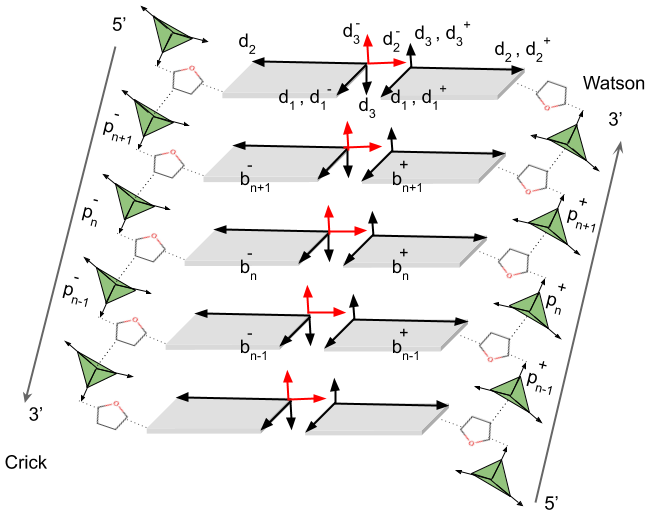
\includegraphics[scale=0.55]{images/Coords.png}
\centering\caption{A schematic view of coarse-grain dsDNA with rigid bases and rigid phosphates. 
The sugar molecule is shown in the image but is modeled only implicitly in the cgDNA$+$ model.
$\{d_1,d_2,d_3\}$ is the orthonormal frame as per Tsukuba convention~\cite{tsukuba} while for modeling purposes we flip the Crick frame to align with Watson frame to give the final orientations of Watson and Crick frame as $\{d_1^+,d_2^+,d_3^+\} \and \{d_1^-,d_2^-,d_3^-\}$, respectively.  
}
\label{c2:fig2}
\end{center}
\end{figure}

This frame fitting leads to a reference point $\v r$ and a right-handed, orthonormal frame $\R^{3 \times 3} \ni D = \{d_1,d_2,d_3\}$ to each base as per Tsukuba convention~\cite{tsukuba}. 
The vector $d_1$ is in the direction of major-groove, $d_2$ in the direction of the reference strand or away from the complementary base and, $d_3 = d_1 \times d_2$ and is approximately in the direction pointing from base $n$ to $n+1$ while reading from that strand.
It implies that the frames associated with the two bases in a given base-pair are not aligned, as shown in \cref{c2:fig2} in black color and denoted as $\{d_1,d_2,d_3\}$.
However, in the context of dsDNA modeling, it is convenient to model if both bases in the base-pair %$d_3$
are aligned in the same direction.
Therefore, we have introduced a matrix $P_\text{{flip}} \in O(3)$,
\begin{equation}
P_\text{{flip}} = 
\begin{bmatrix}
1 & 0 & 0\\
0 &-1 & 0\\
0 & 0 & -1\\
\end{bmatrix}
\label{flipmat}
\end{equation}
which flips $d_2$ and $d_3$ directions of Crick frame. 
It gives the final orientation of Crick frame as $D^{-} = DP_\text{{flip}}=\{d_1,-d_2,-d_3\}=\{d_1^-,d_2^-,d_3^-\}$ and Watson frame as $D^{+} = D = \{d_1,d_2,d_3\}=\{d_1^+,d_2^+,d_3^+\}$.
Now, $d_1^{\pm},d_2^{\pm}, \and d_3^{\pm}$ are in the direction of major-groove, Watson (chosen as reading) strand, and $n$ to $n+1$ base while reading from the Watson strand, respectively.  
Note that after flipping base frames associated with the Crick strand, we have denoted base and phosphate frames on the Watson strand (chosen as the reading strand) with $+$ superscript and on the Crick strand with $-$ superscript.

Similarly, we have defined the 
position of phosphate atom as the reference point, $r^{p} \in \R^3$ and 
three vectors, $\R^{3 \times 3} \ni D^{p} = \{d_{1}^{p},d_{2}^{p},d_{3}^{p}\}$ in the direction of $d_{3}^{p}= \text{O5}' - \text{O3}'$, 
$d_{2}^{p}= \text{P} - (\text{O5}' + \text{O3}')/2$ and, $d_{1}^{p}=d_{2}^{p} \times d_{3}^{p}$.
More details on the ideal coordinates for the phosphate are in \cref{a1:t1}. 
A schematic diagram of coarse-grain bases and phosphates is shown in \cref{c2:fig2}. 
%%%%%%%%%%%%%%%%%%%%%%%%%%%%%%%%%%%%%%%%%%%%%%%%%%%%%%%%%%%%%%%%
%%%%%%%%%%%%%%%%%%%%%%%%%%%%%%%%%%%%%%%%%%%%%%%%%%%%%%%%%%%%%%%%
%%%%%%%%%%%%%%%%%%%%%%%%%%%%%%%%%%%%%%%%%%%%%%%%%%%%%%%%%%%%%%%%
%%%%%%%%%%%%%%%%%%%%%%%%%%%%%%%%%%%%%%%%%%%%%%%%%%%%%%%%%%%%%%%%
%%%%%%%%%%%%%%%%%%%%%%%%%%%%%%%%%%%%%%%%%%%%%%%%%%%%%%%%%%%%%%%%
%%%%%%%%%%%%%%%%%%%%%%%%%%%%%%%%%%%%%%%%%%%%%%%%%%%%%%%%%%%%%%%%
\section{Internal coordinates}\label{c2:sec2}
\begin{figure}[htb]
\begin{center}
%left bottom right top
\centering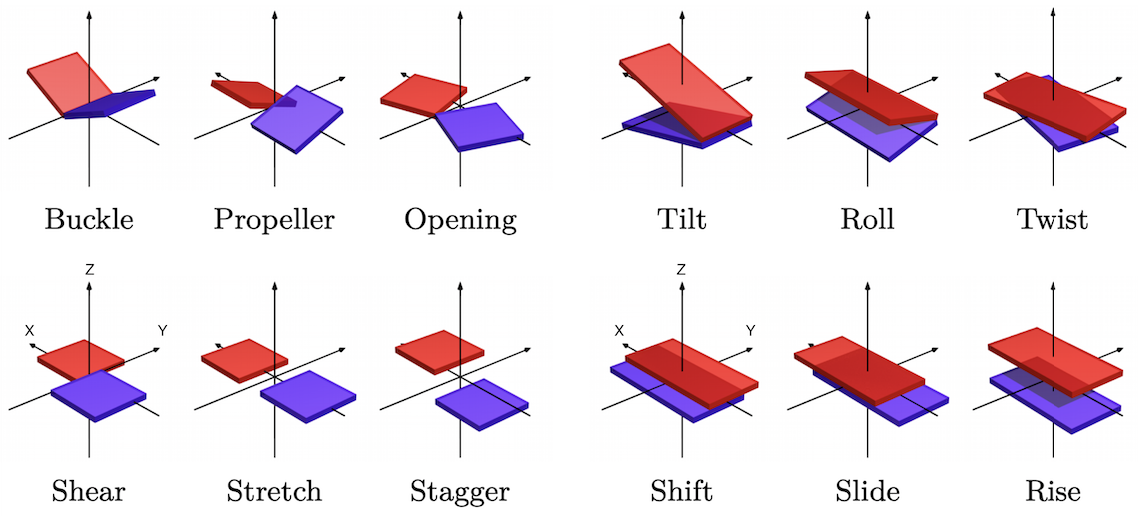
\includegraphics[scale=0.65]{images/IC.png}
\centering\caption{
CURVES$+$ coordinates for a coarse-grain DNA configuration. Intra base-pair (left) and Inter base-pair (right).
X, Y, and Z are in the direction of the reading strand, major-groove, and from base n to n + 1 while reading the sequence from the reference strand, respectively.
}
\label{c2:fig_IC}
\end{center}
\end{figure}

The frames obtained in the last section are in absolute coordinates, i.e., in a fixed lab frame, which are challenging to work with due to global
translations and rotations of the whole molecule during the MD simulation.
A convenient alternative is to use a coordinate system fixed on the dsDNA molecule itself, i.e., internal coordinates. 
In the following discussion, we have first introduced the internal coordinates for the bases and then for the phosphates while reading the sequence ($5^\prime \ \text{to} \ 3^\prime$ direction) from a chosen strand.
The cgDNA$+$ internal coordinates for the same configuration while reading the sequence from two different strands are different but related by a linear transformation. This linear transformation for change of reading strand is reviewed in \cref{c2:sec3sb1}.
Furthermore, the inverse transformation from cgDNA$+$ internal coordinates to the absolute frames is detailed in \cref{c2:s2sb2}.
Lastly, we discussed H-bond filtering to discard MD snapshots with broken H-bonds.

\subsection{Frames to cgDNA$+$ internal coordinates}\label{c2:fra_to_int}
We first defined the base-pair and the junction frames to introduce internal coordinates for bases. The base-pair frame is defined as the average orientation ($B$) of two complementary base frames of a base-pair with an average reference point, $g$ (\cref{c2:eq2}). While the junction frame is defined as the average orientation ($J$) of the two neighboring base-pair frames ($n^\text{{th}}$ and $(n+1)^\text{{th}}$) with average reference point $t$ given in \cref{c2:eq3}.
\begin{equation}
\{ B_n,g_n \} = \{ D_{n}^{-}\sqrt{\Lambda_{n}} \; , \;  \frac{1}{2}(r_{n}^{+} + r_{n}^{-}) \} \;\;\; \text{where} \;\;\; \Lambda_{n} = (D_{n}^{-})^{T}D_{n}^{+}
\label{c2:eq2}
\end{equation}
\begin{equation}
\{ J_n,t_n \} = \{ B_{n}\sqrt{\Gamma_{n}} \; , \;  \frac{1}{2}(g_{n+1} + g_{n}) \} \;\;\; \text{where} \;\;\; \Gamma_{n} = (B_{n})^{T}B_{n+1}
\label{c2:eq3}
\end{equation}
where $\Lambda_{n}$ describes the relative orientation of the base frame $D_{n}^{+}$ with respect to $D_{n}^{-}$ and $\Gamma_{n}$ describes the relative orientation of base-pair frame $B_{n+1}$ with respect to $B_{n}$. 

Now, the internal coordinates for the bases are classified into intra and inter base-pair coordinates.
The rotational components of intra base-pair coordinates are defined as Cayley parameters (refer appendix \cref{a3:s2}) of the relative rotation matrix $\Lambda_{n}$ and the intra translational coordinates, $\zeta_{n}$ are defined in the reference frame of base-pair frame $B_n$ (\cref{c2:eq2}) and are given as,
\begin{equation}
\R^6 \ni \textit{x}_n = \{ \lambda_{n},\; \zeta_{n}\} = \{ cay_{\alpha}^{-1}(\Lambda_{n}),\; B_{n}^{T}(r_{n}^{+}-r_{n}^{-})\}
\label{c2:eq4}
\end{equation}
where $\lambda_{n} \; \text{and} \; \zeta_{n} \in \R^3$ and 
$cay_{\alpha}^{-1}(\cdot)$ is defined in appendix \cref{a3:eq6} and $\alpha \in \R$ is a scaling parameter which is discussed later in this section. 
For the cgDNA$+$ model, we have chosen $\alpha =5$. 
The inter base-pair coordinates are defined between two neighboring base-pairs. 
The rotational component $\gamma_{n} \in \R^3$ is the Cayley parameters of the relative rotation matrix $\Gamma_{n}$ between $n^\text{{th}}$ and $(n+1)^\text{{th}}$ base-pairs. 
While the translational coordinates $\eta_{n} \in \R^3$ are defined as the relative translation between two neighboring base-pair frames but in reference of the junction frame $J_n$. 
The inter base-pair coordinates are given as, 
\begin{equation}
\R^6 \ni \textit{y}_n =  \{ \gamma_{n},\; \eta_{n}\} = \{ cay_{\alpha}^{-1}(\Gamma_{n}),\; J_{n}^{T}(g_{n+1}-g_{n})\}.
\label{c2:eq5}
\end{equation}
Notably, intra rotational and translational coordinates are commonly known as (Buckle, Propeller, Opening) and (Shear, Stretch, Stagger), respectively, and inter rotational and translational coordinates are commonly known as (Tilt, Roll, Twist) and (Shift, Slide, Rise), respectively.
A schematic diagram for intra and inter coordinates is depicted in \cref{c2:fig_IC}.

The internal coordinates for a given phosphate are defined relative to the base to which the phosphate is attached.
It can be defined in two ways: base to $3^\prime-$ phosphate and base to $5^\prime-$ phosphate.
cgDNA$+$ model adopts base to $5^\prime-$ phosphate as this parameterization is through the covalent bond between base and phosphate, which involves B\rom{1}-B\rom{2} backbone conformations.
Both parameterizations were investigated in ref.~\cite{patelithesis} with the findings that base to $5^\prime-$ phosphate parameterization can capture bi-modality in the backbone conformation.
This parameterization is essentially defining coordinates for the phosphate with respect to the corresponding base in the same nucleotide.
More details about the choice of parameterization can be found in A. Patelli's thesis~\cite{patelithesis}.
Finally, the internal coordinates for phosphate are defined in reference to the corresponding base and are given as
\begin{equation}
\R^6 \ni \textit{z}_n^{\pm}= \{\tau_{n}^{\pm},\; \xi_{n}^{\pm}\} = \{ cay_{\alpha}^{-1}(D_{n}^{\pm}D_{n}^{p\pm}),\; D_{n}^{\pm}^{T}(r_{n}^{p\pm}-r_{n}^{\pm})\}.
\label{c2:eq6}
\end{equation}

Thus, the coarse-grain  configuration of dsDNA oligomer of length $N$ bps in terms of internal coordinates (independent of global translation and rotation of the molecule) can be written as a vector $w$ in $24N-18$ dimensions made up of $6N$ intra base-pair ($\textit{x}_n$), $6N-6$ inter base-pair ($\textit{y}_n$) and $12N-12$ base to $5^\prime-$phosphate coordinates ($\textit{z}_n^{\pm}$) given in \cref{c2:eq7},
\begin{equation}
\R^{24N-18} \ni w = (\textit{x}_1,\textit{z}_1^{-},\textit{y}_1,\textit{z}_2^{+}, \textit{x}_2,\textit{z}_2^{-},....,\textit{y}_{n-1},\textit{z}_n^{+}, \textit{x}_n),
\label{c2:eq7}
\end{equation}
where $\pm$ denote Watson and Crick strands, respectively. 
The transformations in \cref{c2:eq2,c2:eq3,c2:eq4,c2:eq5,c2:eq6} that transform bases and phosphates frames into internal coordinates for a given dsDNA configuration is denoted by $T_{F\xrightarrow{}I} : SE(3)^{4N-2} \xrightarrow{} \R^{24N-18}$.

Lastly, we have chosen a scale of 1 \AA \ for translational coordinates and rad/5 for rotational coordinates and transformed the coordinates into dimensionless form and scaled them so that the magnitudes of the rotational and translational coordinates can be compared more directly. 
More details on the scaling parameters can be found in refs.~\cite{petthesis,cgDNA1,petkevivciute2014cgdna}.

\subsection{Change of reading strand}\label{c2:sec3sb1}
In the previous section, we introduced cgDNA$+$ internal coordinates to describe the configuration of dsDNA while reading the sequence from a particular strand (chosen first).
However, the same dsDNA configuration read from the Watson strand ($\sq$) or the Crick strand ($\bar{\sq}$) leads to two different cgDNA$+$ internal coordinates, which are related by a linear map~\cite{petthesis,patelithesis} as,
\begin{equation}
\begin{split}
w(\bar{\sq}) &= E_{N}w(\sq)\\
\K(\bar{\sq})&= E_{N}\K(\sq)E_{N}
\end{split}
\label{changereadstrand}    
\end{equation}
where
\begin{equation}
\R^{24N-18\times24N-18} \ni E_{N} =  
\begin{bmatrix}
&&&&&E^{5^\prime} \\
&&&E^{int}&& \\
&& \reflectbox{$\ddots$} &&& \\
&E^{int}&&&& \\
E^{3^\prime}&&&&& \\
\end{bmatrix}
\label{Etot}
\end{equation}
and $\K$ is the stiffness matrix discussed in \cref{c2:sec3}.
The entries in $E_N$ are given as
\begin{equation}
\R^{36\times36} \ni E^{5^\prime}%,E^{3^\prime}  
= 
\begin{bmatrix}
&&&&&E \\
&&&&I_6& \\
&&&E&& \\
&&I_6&&& \\
&E&&&& \\
I_6&&&&& \\
\end{bmatrix}, 
% \begin{bmatrix}
% &&&&&I_6 \\
% &&&&E& \\
% &&&I_6&& \\
% &&E&&& \\
% &I_6&&&& \\
% E&&&&& \\
% \end{bmatrix}
\label{Emat53}
\end{equation}
\begin{equation}
\R^{36\times36} \ni E^{3^\prime} =  [E^{5^\prime}]^{-1} = [E^{5^\prime}]^T , \and
\label{Emat53}
\end{equation}

\begin{equation}
\R^{42\times42} \ni E^{int} =  
\begin{bmatrix}
&&&&&&I_6 \\
&&&&&E& \\
&&&&I_6&& \\
&&&E&&& \\
&&I_6&&&& \\
&E&&&&& \\
I_6&&&&&& \\
\end{bmatrix}
= [E^{int}]^T= [E^{int}]^{-1}
\label{Ematint}
\end{equation}
where $E = \text{diag}(-1,1,1,-1,1,1) \in \R^{6\times6}$ and $I_6$ is a $6\times6$ identity matrix. 

\subsection{cgDNA$+$ internal coordinates to frames}\label{c2:s2sb2}
The inverse transformation to obtain the position and orientation of base and phosphate frames from cgDNA$+$ internal coordinates is denoted as $T_{I\xrightarrow{}F} : \R^{24N-18}  \xrightarrow{} SE(3)^{4N-2}$.
%$T_{I\xrightarrow{}F}$ fits the frames in any cgDNA$+$ configuration.% and then re-embeds the ideal coordinates to fine-grain the cgDNA$+$ configuration to obtain the PDB structure with atomistic coordinates. 
For a given configuration in cgDNA$+$ internal coordinates,
$w = (\textit{x}_1,\textit{z}_1^{-},\textit{y}_1,\textit{z}_2^{+}, \textit{x}_2,\textit{z}_2^{-},\cdot \cdot \cdot \cdot,  \textit{y}_{n-1},\textit{z}_n^{+}, \textit{x}_n)$ $\in \R^{24N-18}$ where each component can further be split into rotational and translational components as $\textit{x}_n = (\lambda_{n},\zeta_{n}), \textit{y}_n = (\gamma_{n}, \eta_{n}), \and \textit{z}_n^\pm =  (\tau_n^\pm, \xi_n^\pm)$, bases and phosphates frames can be obtained in three steps.
First the $n^{\text{th}}$ base-pair frame ($B_n,g_n$) can be obtained from the corresponding inter coordinates ($\textit{y}_{n-1}$) using recursive relation as  
\begin{equation}
\begin{split}
\begin{bmatrix}
B_{n} & g_{n} \\
\v 0^T & 1 
\end{bmatrix} 
&=
\begin{bmatrix}
B_{n-1} & g_{n-1} \\
\v 0^T & 1 
\end{bmatrix} 
\begin{bmatrix}
cay_{\alpha}(\gamma_{n-1}) & cay_{\alpha}(\gamma_{n-1})\eta_{n-1} \\
\v 0^T & 1 
\end{bmatrix} \\
&=
\prod_{i=1}^{n-1}
\begin{bmatrix}
cay_{\alpha}(\gamma_{i}) & cay_{\alpha}(\gamma_{i})\eta_{i} \\
\v 0^T & 1 
\end{bmatrix} 
\end{split}
\end{equation}
where $cay_{\alpha}(\cdot)$ is the Cayley transformation defined in \cref{a3:eq5} with $\alpha$ as the scaling factor discussed in \cref{c2:sec3sb1}, and ($B_1,g_1$) is taken as $( \v I, \v 0 )$ with $\v I \in \R^{3\times 3}$ an identity matrix and $\v 0 \in \R^{3 \times 1}$ a zero vector.
Note that absolute coordinates for frames require a reference point, which is chosen to be the first base-pair frame.
Subsequently, base and phosphate frames can be obtained as
\begin{equation}
\begin{bmatrix}
D_n^{\pm} & r_n^{\pm} \\
\v 0^T & 1 
\end{bmatrix}
 = 
\begin{bmatrix}
 B_n (cay_{\alpha}(\lambda_n))^{\pm\frac{1}{2}} & g_n \pm \frac{1}{2} B_n\zeta_n \\
\v 0^T & 1 
\end{bmatrix}
\end{equation}
\begin{equation}
\begin{bmatrix}
D_n^{p\pm} & r_n^{p\pm} \\
\v 0^T & 1 
\end{bmatrix}
 =
\begin{bmatrix}
D_n^{\pm} L^\pm cay_{\alpha}(\tau_n^{\pm}) & g_n^{\pm} + \frac{1}{2} D_n^{\pm} L^\pm \xi_n^{\pm} \\
\v 0^T & 1
\end{bmatrix}
\end{equation}
where $L^+ = \v I, \and L^- =  
P_\text{{flip}}$ (see \cref{flipmat}).

Lastly, to obtain the atomistic PDB structure one can re-embed ideal atom coordinates (\cref{a1:t1}) in bases and phosphates frames using the transformation $T_{F\xrightarrow{}C}  :  SE(3)\xrightarrow{} \R^{3 \times K}$.
For a given frame with ($R,r$) as orientation and position, the positions of the associated atoms can be obtained as, 
\begin{equation}
\mathcal{C}_{X^k} =: R \mathcal{A}_{X^k} + r, \ \forall \ k = 1 \cdot \cdot K
\label{c2:eq_T_F_C}
\end{equation}
where $K$ is the number of atoms in base or phosphate, $X$ is kind of rigid body (base or phosphate), $\mathcal{A}_{X^k} \in \R^{3 \times 1}$
is the coordinate of $k^{\text{th}}$ ideal atom in $X$ type rigid body, and $\mathcal{C}_{X^k} \in \R^{3 \times 1}$ is the coordinate of $k^{\text{th}}$ atom embedded in the frame.


\subsection{H-bond filtering}\label{c2:sec3sb2}
We have used the Cayley vector to parameterize rotational coordinates between two rigid bodies, whose norm tends to infinity if the relative rotation between the rigid bodies is close to $\pi$. 
This case can happen in MD time-series due to broken H-bonds, especially toward the ends of a dsDNA molecule.
Such cases may lead to massive bias in the statistics of the rotational internal coordinates, which may create optimization issues in model training.
Moreover, MD snapshots after broken H-bond filtering may better represent the dsDNA properties than the raw data. 
Thus, we have introduced a filtering step that removes snapshots with one or more broken H-bonds.
We have declared (consistent with~\cite{cgDNA1,petkevivciute2014cgdna,lankavs2009parameterization,3dna}) an H-bond broken if a) distance between the heavy atoms involved in the H-bond is greater than four \AA \ or b) the angle between the heavy atoms via H-atom is less than $120^\circ$. 
The latter condition, in general, can not be applied to dsDNA data obtained from X-ray techniques (as the H atom is missing); therefore, only the first criterion is used~\cite{3dna}.
%%%%%%%%%%%%%%%%%%%%%%%%%%%%%%%%%%%%%%%%%%%%%%%%%%%%%%%%%%%%%%%%
%%%%%%%%%%%%%%%%%%%%%%%%%%%%%%%%%%%%%%%%%%%%%%%%%%%%%%%%%%%%%%%%
%%%%%%%%%%%%%%%%%%%%%%%%%%%%%%%%%%%%%%%%%%%%%%%%%%%%%%%%%%%%%%%%
%%%%%%%%%%%%%%%%%%%%%%%%%%%%%%%%%%%%%%%%%%%%%%%%%%%%%%%%%%%%%%%%
%%%%%%%%%%%%%%%%%%%%%%%%%%%%%%%%%%%%%%%%%%%%%%%%%%%%%%%%%%%%%%%%
%%%%%%%%%%%%%%%%%%%%%%%%%%%%%%%%%%%%%%%%%%%%%%%%%%%%%%%%%%%%%%%%
\section{cgDNA$+$ model}\label{c2:sec3}
cgDNA$+$ model is a predictive model that given a sequence $\sq$ of length $N$ bps along the reading strand and a parameter set $\mathcal{P}$ delivers a Gaussian pdf in configuration space by reconstructing a ground-state $\hat{w} (\sq, \mathcal{P}) \in \R^{24N-18}$ and a positive-definite stiffness matrix $\K (\sq, \mathcal{P}) \in \R^{24N-18 \times 24N-18}$:
\begin{equation}
\rho(w; \sq, \mathcal{P}) = \frac{1}{\textit{Z}} exp \{-\frac{1}{2}(w-\hat{w})\cdot \K (w-\hat{w})\}.
\label{c2:eq8}
\end{equation}

In cgDNA$+$ model, a parameter set $\mathcal{P}$ for dsDNA in standard alphabets is made up of a) ten independent interior dinucleotide-dependent $\K^{\XY}$  blocks $\in \R^{42 \times 42}$ plus sixteen independent $\K^{5^\prime\XY}$ end blocks $\in \R^{36 \times 36}$, and b) ten independent interior dinucleotide-dependent stress vectors $\sigma^{\XY} \in \R^{42} $ plus sixteen independent $\sigma^{5^\prime\XY}$ end stress vectors $\in \R^{36}$,
\begin{equation}
\mathcal{P} = \{ \sigma^{5^\prime\XY},  \sigma^{\XY}, \K^{5^\prime\XY}, \K^{\XY} \} \in
\P = [\R^{36}]^{16} \times [\R^{42}]^{10} \times [\R^{36 \times 36}]^{16} \times [\R^{42 \times 42}]^{10},
\label{c2:eq9}
\end{equation}
where $5^\prime\XY \in\{16$ dimer steps$\}$ and $\XY \in\{10$ independent dimer steps$\}$. The parameter for $3^\prime$ ends and dependent dimer steps can be obtained using Crick-Watson (CW) symmetry as; 
\begin{equation}
\begin{split}
\sigma^{\bar{\text{Y}}\bar{\text{X}}}  &= E^{int}\sigma^{\XY}\\
\K^{\bar{\text{Y}}\bar{\text{X}}} &=  E^{int}\K^{\XY}E^{int}  \\
\sigma^{\bar{\text{Y}}\bar{\text{X}}3^\prime}  &= E^{5^\prime}\sigma^{5^\prime\XY}\\
\K^{\bar{\text{Y}}\bar{\text{X}}3^\prime} &=  E^{5^\prime}\K^{5^\prime\XY}E^{5^\prime}  \end{split}
\label{c2:eq_CW_in_Prm}    
\end{equation}
Note that these symmetry conditions put additional constraints on the parameter blocks for palindromes X$\bar{\text{X}}$ (AT, TA, CG, and GC for dsDNA), which are exploited in the parameter set extraction. 
The details on the parameter set estimation are provided in \cref{c2:sec4}.
 
\subsection{cgDNA$+$ model assumptions}\label{c2:s3_assump}
The assumptions or approximations in the cgDNA$+$ model are the following:
\begin{itemize}
\label{c2:list1}
    \item[i)] MD time-series are stationary 
    \item[ii)] base and phosphates are rigid
    \item[iii)] pdfs of internal coordinates follow Gaussian distribution, i.e., internal energy for any oligomer assumes a shifted quadratic (see \cref{c2:eq8})
%    \item y
    \item[iv)] total energy of the dsDNA oligomer is approximated as the sum of local junction energies, i.e., nearest-neighbor interactions only,  
    \begin{equation}
    U(w,\sq) = \frac{1}{2}(w-\hat{w}).\K (w-\hat{w})
\approx \frac{1}{2}\sum_{n=1}^{N-1}
    (w_n-\hat{w}_n).\K_n (w_n-\hat{w}_n)
    \label{c2:eq_sum_of_energy} 
    \end{equation}
    where $w_n, \hat{w}_n, \and \K_n$ represents local junction energy contribution.
    \item[v)] coefficients in the local junction energies depend on the local dimer step.
\end{itemize}

\begin{figure}[htb]
\begin{center}
\centering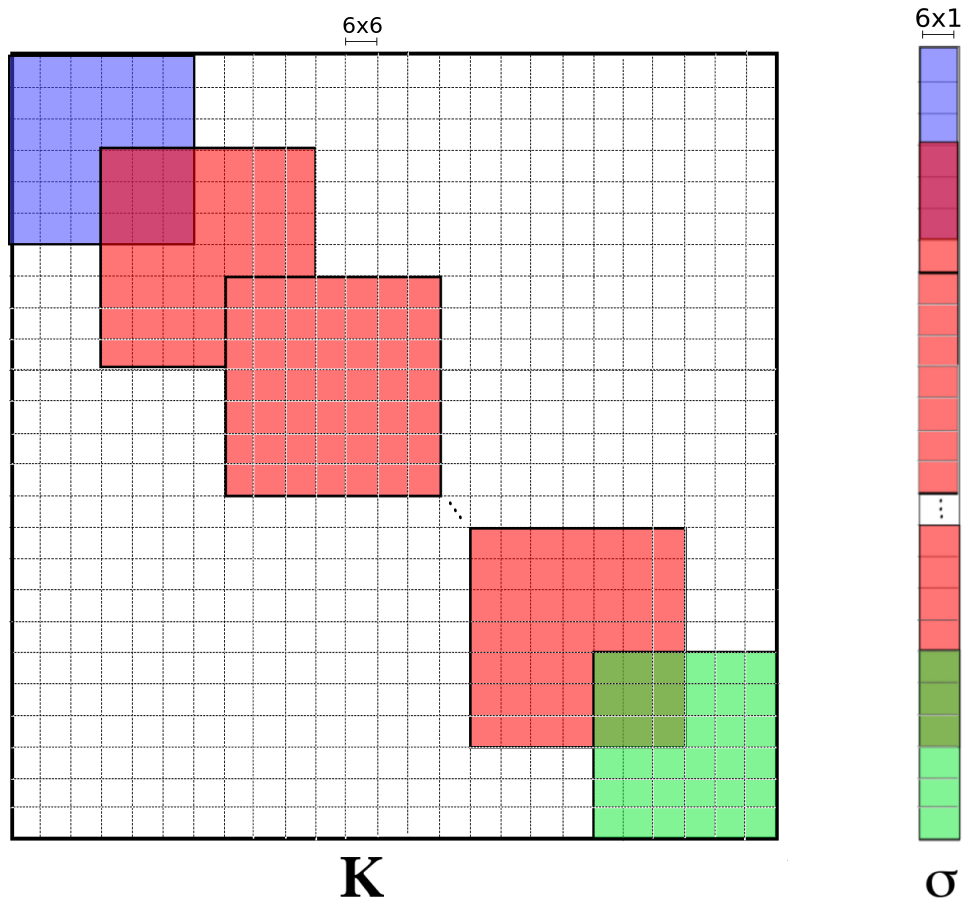
\includegraphics[scale=0.26]{images/combine_matrix.png} %,trim = 0cm 2.5cm 0cm 0cm
\centering\caption{
Construction of banded oligomer stiffness matrix $\K$ and stress vector $\sigma$ by overlapping dimer-step dependent parameter set blocks shown for poly(A).
The parameters for $3^\prime$ end, $5^\prime$ end, and interior blocks are different and are shown in different colors.
Each cell of the matrix is of dimension $6\times 6$. Each cell in the vector is of dimension $6\times1$.
}
\label{c2:fig3}
\end{center}
\end{figure}

Solving \cref{c2:eq_sum_of_energy} with appropriate algebraic considerations (for more details refer~\cite{petthesis}), the groundstate for the dsDNA oligomer is given as
\begin{equation}
\hat{w}(\sq) = \K^{-1}(\sq)\sigma(\sq)
\label{c2:eq10}
\end{equation}
where $\K(\sq) \and \sigma(\sq)$ can be computed by overlaying dimer-dependent parameter blocks (as shown in \cref{c2:fig3} and discussed in \cref{c2:sec3sb2}) and $\sigma_n = \K_n\hat{w}_n$.
It leads to one of the most important features in the cgDNA$+$ model; that is, even though $\K$ matrix and $\sigma$ vector have local sequence dependence, the groundstate configuration which involves the inversion of overlapping banded stiffness matrix ($\K$) has a non-local (often strongly non-local) sequence dependence. 
Moreover, a non-zero constant energy term $\hat{U}(\sq)$ naturally arises in the solution of \cref{c2:eq_sum_of_energy} reflecting that all bases and phosphates cannot simultaneously achieve absolute zero energy minima in the ground–state and achieve an equilibrium configuration with some non-zero frustration energy.
This physical phenomenon of frustration observed here is only possible in double chain rigid base model (cgDNA) or higher hierarchy models like cgDNA$+$ but not in single-chain models such as rigid base-pair models.

\subsection{cgDNA$+$ reconstruction}\label{c2:s3sb1}
Given a sequence $\sq$ and parameter set $\mathcal{P}$, the model $\K$ matrix and $\sigma$ vector are constructed by overlaying dinucleotide-step parameter set blocks as shown in \cref{c2:fig3} and given as
\begin{equation}
\K(\Pc,\sq) = R_{d}^{T}\K_{d}R_{d} \;\; \text{and} \;\;   \sigma(\Pc,\sq) = R_{d}^{T}\sigma_{d} 
\label{recons}
\end{equation}
where $\K_d = \text{diag}(\K^{5^\prime X_1X_2},...,\K^{X_iX_{i+1}},...,\K^{X_{N-1}X_{N}3^\prime})$ and $\sigma_d = (\sigma^{5^\prime X_1X_2},...,\sigma^{X_iX_{i+1}},...,\sigma^{X_{N-1}X_{N}3^\prime})$
and $R_{d} \in 42N-12 \times 24N-18$ is a matrix defined in \cref{reconsmat}. 
\begin{equation}
R_{d} = \begin{bmatrix}
   I_{18} &  & &  & & \dots & &\\
   & I_{18} & &  & &  & & \\
   & I_{18} & &  & &  & & \\
   & & I_{6}  &  & &  & & \\
   &  & & I_{18} & &  & & \\
   &  & & I_{18} & &  & & \\
   &  & &  &I_{6} &  & & \\
  \vdots & & &  & &\ddots  & &\vdots \\
      &  & &  & &  & &I_{18} \\
 \end{bmatrix}
\label{reconsmat}
\end{equation}
where $I_k$ is k-dimensional identity matrix. 

Thus, given a sequence $\sq$ and parameter set $\Pc$, we can define a reconstruction rule $\Rc(\Pc,\sq)$ which reconstructs a banded stiffness matrix $\K(\sq)$ and a $\sigma(\sq)$ vector as
\begin{equation}
\Rc(\Pc,\sq) = (\sigma(\Pc,\sq),\K(\Pc,\sq)).
\label{reconsmap}    
\end{equation}
It is important to note that the reconstruction rule $\Rc(\Pc,\sq)$ is not invertible due to overlapping blocks in the stiffness matrix $\K$ and stress vector $\sigma$.

Moreover, we have defined $\Rc_{\text{vec}}(\Pc_\text{vec},\sq)$ which is equivalent to $\Rc(\Pc,\sq)$ but allows a linear relation between $\sigma(\Pc,\sq)$, $\K(\Pc,\sq)$ and the vector form of parameter set $\Pc_\text{vec} \in \R^{L}$ where L is the total number of independent entries in the parameter set $\Pc$. 
It can be defined as
\begin{equation}
\Rc_{\text{vec}}(\Pc_\text{vec},\sq) = R_{\Pc}(\sq)\Pc_\text{vec}= (\sigma(\Pc,\sq),\K(\Pc,\sq) )
\label{reconsmap2}    
\end{equation}
where $R_{\Pc}(\sq) \in N+N^2 \times L$ is parameter reconstruction matrix which maps the entries in parameter set in vector form $\Pc_\text{vec}$ to the entries of $\sigma(\sq)$ and $\K(\sq)$.
This vectorized form is convenient to code and explain the mathematics of extracting the cgDNA$+$ parameter set.\clearpage
%%%%%%%%%%%%%%%%
%%%%%%%%%%%%%%%%%%%%%%%%%%%%%%%%%%%%%%%
%%%%%%%%%%%%%%%%%%%%%%%%%%%%%%%%%%%%%%%%%%%%
%%%%%%%%%%%%%%%%%%%%%%%%%%%%%%%%%%%%%%%
%%%%%%%%%%%%%%%%%%%%%%%%%%%%%%%%%%%%%%%%%%%%
%%%%%%%%%%%%%%%%%%%%%%%%%%%%%%%%%%%%%
%%%%%%%%%%%%%%%%%%%%%%%%%%%%%%%%%%%%%%%%%%%%%%
\section{cgDNA$+$ parameter set estimation}\label{c2:sec4}
In this section, we have discussed the protocol for extraction of cgDNA$+$ model parameter set from MD time-series. 
This protocol was initially developed for the cgDNA model~\cite{petkevivciute2014cgdna} and was optimized and extended for the cgDNA$+$ model~\cite{patelithesis}. 
The key steps in this protocol are:
\begin{itemize} \label{c2:list2}
\setlength\itemsep{0em}
    \item[i)] long-enough atomistic MD time-series for a set of sequences referred to as the training library, Lb (discussed in \cref{c3:s3})
    \item [ii)] fit rigid bodies in atomistic MD snapshots to obtain snapshots in base and phosphate frames as discussed in \cref{c2:sec1} and discard snapshots with broken H-bond.
    \item [iii)] transform base and phosphate frames into internal coordinates using $T_{F\xrightarrow{}I}$ (see \cref{c2:sec2})
    \item [iv)] estimation of first and second moments (i.e., fit Gaussian pdf) for each oligomer in the training library, assuming that MD time-series are converged (\cref{c2:s4:sb1}).
    \item [v)] train dimer-dependent $\sigma$ vector and $\K$ stiffness matrix (i.e., parameter set $\Pc$ as defined in \cref{c2:eq9}) using Gaussian pdfs obtained in the previous step. This step is explained in \cref{c2:s4:sb3,c2:s4:sb4,c2:s4:sb5}
    \item [vi)] parameter set stiffness blocks obtained in last step may not be positive-definite, so search an element in null space to make stiffness blocks positive-definite (see \cref{c2:s4:sb6}).
\end{itemize}
All the above steps in the parameter set estimation are briefly discussed in the following subsections and a detailed explanation can be found elsewhere~\cite{patelithesis}. 
%%%%%%%%%%%%%%%%%%%%%%%%%%%%%%%%%%%%
%%%%%%%%%%%%%%%%%%%%%%%%%%%%%%%%%%%%
\subsection{Estimation of oligomer-level statistics} \label{c2:s4:sb1}
Once the internal coordinates are obtained for each MD snapshot for all sequences in the training library (Lb $=\{\sq_i\}_{i=1}^{L}$), the next step is to compute oligomer-level statistics, $\{\bar{w}(\sq),C(\sq)\}$.  
For a given MD time-series ($\left[w^m(\sq)\right]_{m=1}^{M}$) where $m$ represents the $m^{th}$ snapshot in the time-series and $M \sim 10^6$ is the total number of snapshots in the time-series, the first moment (mean) and second central moment (covariance matrix) can be computed as,
\begin{equation}
\label{estimator}
\begin{split}
\bar{w}(\sq) &= \frac{1}{M} \sum_{m=1}^M w^m(\sq) \\ C(\sq) &= \frac{1}{M} \sum_{m=1}^M \left(w^m(\sq) - \bar{w}(\sq)\right) \left(w^m(\sq) - \bar{w}(\sq)\right)^T \; \forall \; \sq \in \Lb.
\end{split}
\label{c2:eq_moments}
\end{equation}
Furthermore, we have exploited the CW symmetry of dsDNA (only if the sequence is a palindrome, i.e., $\sq = \bar{\sq}$) to enhance the quality of first and second centred moments by defining palindromically symmetrized estimators
as:
\begin{equation}
\label{palinestimator}
\begin{split}
\bar{w}_p(\sq) &= \frac{1}{2}(\bar{w}+E_{N}\bar{w}) \\ 
H(\sq) & = C + \bar{w}\bar{w}^T\\
H_p(\sq) & = \frac{1}{2}(H+E_{N}HE_{N}) \\
C_p(\sq) & = H_p - \bar{w}_p\bar{w}_p^T
\end{split}
\end{equation}
where $H$ is the second moment and $E_{N}$ defines a linear map for reading strand transformation (refer \cref{c2:sec3sb1}). 
Note that all sequences used to train cgDNA$+$ model parameters are palindromes (see \cref{palinold}).
Therefore, we have dropped the subscript notation for convenience, i.e., $\bar{w}_p(\sq)$ is written as $\bar{w}(\sq)$.
Lastly, the cgDNA$+$ model only considers the first and second moments, as the computation of higher moments in such high dimensions $\in \R^{24N-18}$ is non-trivial. 

Now, the maximum entropy principle~\cite{jaynes1,jaynes2} allows computing the least biased probability distribution
for precise prior data.
The absolute entropy for a density $\rho(w)$ is given as:
\begin{equation}
D(\rho) = - \int_{\R^{24N-18}} \rho(w) \log \rho(w) dx.
\label{c2:eq13}
\end{equation}
By assumption, in our case, the probability distribution is a Gaussian pdf with $\bar{w}(\sq)$ and $C(\sq)$ $\forall \; \sq \in \text{Lb}$ as mean and covariance, respectively.
We have computed the least biased observed Gaussian probability distribution $\rho_{o}(w;\bar{w}(\sq),C(\sq))$ using \cref{c2:eq13} under the following constraint, 
\begin{equation}
\mathcal{C}(\sq) = \left\{ \rho(w)|\langle 1 \rangle_{\rho}=1, \langle w \rangle_{\rho}=\bar{w}, \langle (w-\bar{w})^{T}(w-\bar{w}) \rangle_{\rho}= C  \right\}
\label{c2:eq14}
\end{equation}
Note that using maximum likelihood estimation to find the observed Gaussian pdf would have resulted in the same probability distribution. More details can be found in ref.~\cite{entropy,patelithesis}.

\subsection{Definition of best-fit parameter set} \label{c2:s4:sb3}
In the previous step, we obtained oligomer-level Gaussian pdfs ($\rho_{o}(w;\bar{w}(\sq),C(\sq))$ abbreviated as $\rho_{o}(w;\sq)$) observed in MD time-series for all $\sq \in \Lb$. 
%Now, using these observed Gaussian pdfs, we have trained the cgDNA$+$ model parameter set. 
The best-fit cgDNA$+$ parameter set $\Pc$ to these observed Gaussian pdfs is defined as 
\begin{equation}
\Pc =  \argmin_{\substack \Ptex \in \P} \sum_{i=1}^{L} D_{\text{KL}} (\rho_\Ptex(w;\sq_i, \Ptex)),\rho_{o}(w;\sq_i))
\label{c2:eq17}
\end{equation}
where $L$ is the number of sequences Lb, $D_{\text{KL}}$ is the Kullback-Leibler (KL) divergence defined in \cref{a3:eq12}, $\rho_{o} = \rho_{o}(w; \sq)$ is the observed Gaussian obtained in the previous step from the raw MD data, and $\rho_\Ptex = \rho_\Ptex(w;\Ptex,\sq)$ is
Gaussian pdf predicted by the parameter set ($\Ptex$) for a given sequence.
$\P$ contains all admissible parameter sets for the cgDNA$+$ model in which $\sigma^{\XY}$ and $\K^{\XY}$ satisfy CW symmetry constraints for palindromic dimer steps as described in \cref{c2:eq_CW_in_Prm} and $\K^{\XY}$ reconstructs a positive definite stiffness matrix for any $\sq \in \text{Lb}$. 
Lastly, note that two notations are used for parameter set, $\Pc$ is the best-fit parameter set while $\Ptex$ is any parameter set in $\P$.

Note that KL divergence~\cite{kld} is not symmetric (details in \cref{c2:sec4}), and therefore, there exist two orderings of arguments in \cref{c2:eq17}. 
In the model training, Gaussian predicted by the model (see \cref{c2:eq8}) is in the first argument, while the observed banded Gaussian (in MD simulations) is in the second. The parameter set estimation in this ordering is the maximum entropy estimation of the parameter set.
Swapping the arguments (Maximum Likelihood estimation of the parameter set) has noticeable changes in the parameter set; however, the general predictions from the parameter set obtained from either setting are close. 
Comparison of these choices is not the main focus of this thesis, and a detailed discussion on this will be published elsewhere. \clearpage

\subsection{Computation of initial solution for the parameter set}\label{c2:s4:sb4}
The next step is to numerically solve \cref{c2:eq17} which requires an initial guess solution for the parameter set.
This section briefly describes how to obtain the initial guess solution using the Fisher information matrix, and more details can be found elsewhere~\cite{patelithesis}. 

The Fisher information~\cite{fisher} can be defined as the second centred moment of $\log{\rho(x;\theta)}$ conditional to parameter $\R^N \ni \theta = \{\mu,\K\}, \; N > 1$, 
\begin{equation}
\left[\F(\theta)\right]_{ij} = -\mathbb{E}\Bigg[\frac{\partial^2}{\partial\theta_i\partial\theta_j}(\log{\rho(x;\theta)})\bigg{|} \theta \bigg]
    \label{fishinfo2}
\end{equation}
where $\rho(x;\theta)$ is a pdf conditional on parameter $\theta \in \R^N$, and $\mu$ and $\K$ are the mean and inverse covariance matrix.   
Furthermore, for two parametric pdfs that are close in parametric space, say
$\rho(x;\theta') $ and $ \rho(x;\theta)$ where $\theta = \theta'+\delta\theta$,  $\;\theta,\; \theta', \; \delta\theta \in \R^N \; \text{and} \; \delta\theta <<1$, there exists a relation between KL divergence (defined in appendix \cref{a3:s4}) and Fisher information, 
\begin{equation}
\F(\theta) = -\int_{\Omega} \rho(x,\theta')\frac{\partial^2}{\partial\theta'^2}\log(\rho(x,\theta')) = \frac{\partial^2}{\partial\theta^2}D_{\text{KL}}(\rho(x,\theta'),\rho(x,\theta))\big|_{\theta=\theta'}.
\label{KLfish1}
\end{equation}
Now, using Taylor expansion at $\theta=\theta'$ gives, 
\begin{equation}
D_{\text{KL}}(\rho(x;\theta'), \rho(x;\theta)) = \frac{1}{2}\delta{\theta}.\F(\theta)\delta{\theta} + \mathcal{O}(|\delta{\theta}^3|) = D_{\text{KL}}(\rho(x;\theta),\rho(x;\theta')).
\label{KLfish2}
\end{equation}
The training of cgDNA$+$ model (refer \cref{c2:eq17}) requires computation of the KL divergence between the observed Gaussian for each oligomer in the training library, $\rho(w;\theta_{o}(\sq))$ and banded Gaussian predicted by cgDNA$+$ reconstruction, $\rho(w;\theta_{\Ptex_\text{vec}}(S,\Ptex))$. 
Now, \cref{KLfish2} can be approximated as, 
\begin{equation}
D_{\text{KL}}(\rho(w;\theta_{\Ptex_\text{vec}}), \rho(w;\theta_{o})) \approx \frac{1}{2}\theta_{\Ptex_\text{vec}}.\F(\theta_{o})\theta_{\Ptex_\text{vec}}- \theta_{\Ptex_\text{vec}}.\F(\theta_{o})\theta_{o} + \frac{1}{2}\theta_{o}.\F(\theta_{o})\theta_{o}
\label{KLfish3}
\end{equation}
Using the relation $\theta_{\Ptex_\text{vec}}(\Ptex,\sq) = R_{\Ptex}(\sq)\Ptex_\text{vec} $ (\cref{reconsmap2}) in \cref{KLfish3} gives, 
\begin{equation}
\begin{split}
D_{\text{KL}}(\rho(w;\theta_{\Ptex_\text{vec}}), \rho(w;\theta_{o})) \approx& \frac{1}{2}\Ptex_\text{vec}.R_{\Ptex}^{T}(\sq)\F(\theta_{o})R_{\Ptex}(\sq)\Ptex_\text{vec}\\ & -\frac{1}{2}\Ptex_\text{vec}.R_{\Ptex}^{T}(\sq)\F(\theta_{o})\theta_{o} + \frac{1}{2}\theta_{o}.\F(\theta_{o})\theta_{o}.
\end{split}
\label{KLfish4}
\end{equation}
Now, using linear change of variable $\F_{(\Ptex,\sq)}(\theta_{o})=R_{\Ptex}^{T}(\sq)\F(\theta_{o})R_{\Ptex}(\sq)$ in above equation gives 
\begin{equation}
\begin{split}
D_{\text{KL}}(\rho(w;\theta_{\Ptex_\text{vec}}), \rho(w;\theta_{o})) \approx& \frac{1}{2}\Ptex_\text{vec}.\F_{(\Ptex,\sq)}(\theta_{o})\Ptex_\text{vec}\\ & - \frac{1}{2}\Ptex_\text{vec}.R_{\Ptex}^{T}(\sq)\F(\theta_{o})\theta_{o} + \frac{1}{2}\theta_{o}.\F(\theta_{o})\theta_{o}.
\end{split}
\label{KLfish5}
\end{equation}
Now, in order to find the best-fit parameter set, the following equation needs to be minimized,
\clearpage

\begin{equation}
\begin{split}
\sum_{i=1}^{L}D_{\text{KL}}(\rho(w;\theta_{\Ptex_\text{vec}}(\sq_i)),& \rho(w;\theta_{o}(\sq_i))) \approx 
\sum_{i=1}^{L}\frac{1}{2}\Ptex_\text{vec}.\F_{(\Ptex,\sq_i)}(\theta_{o})\Ptex_\text{vec}\\ & - \sum_{i=1}^{L}\frac{1}{2}\Ptex_\text{vec}.R_{\Ptex}^{T}(\sq_i)\F(\theta_{o})\theta_{o} + \sum_{i=1}^{L}\frac{1}{2}\theta_{o}.\F(\theta_{o})\theta_{o}.
\end{split}
\label{initialsol2}
\end{equation}
Thus, differentiating \cref{initialsol2} with respect to  $\Ptex_\text{vec}$ gives,
\begin{equation}
\begin{split}
\sum_{i=1}^{L}\F_{(\Ptex,\sq_i)}(\theta_{o})\Ptex_\text{vec} - \sum_{i=1}^{L}R_{\Ptex}^{T}(\sq_i)\F(\theta_{o})\theta_{o} = 0,
\end{split}
\label{initialsol3}
\end{equation}
which can be solved using the least squares method. \Cref{initialsol3} can be rewritten as 
\begin{equation}
\begin{split}
&\F_{(\Ptex,\Lb)}\Ptex_\text{vec} = B \\
&\text{where} \; \F_{(\Ptex,\Lb)} = \sum_{i=1}^{L}\F_{(\Ptex,\sq_i)}(\theta_{o}), B = \sum_{i=1}^{L}R_{\Ptex}^{T}(\sq_i)\F(\theta_{o})\theta_{o}.
\end{split}
\label{initialsol4}
\end{equation}
However, the matrix $\F_{(\Ptex,\Lb)}$ is not invertible due to non-injectivity of the reconstruction rule (\cref{c2:s3sb1}). 
Therefore, to find the least squares solution for \cref{initialsol4}, Moore-Penrose pseudo-inverse has been used to obtain the initial guess as
\begin{equation}
\begin{split}
\Pc_\text{vec}^{\text{lsq}} = \F_{(\Ptex,\Lb)}^{\dagger}B, 
\end{split}
\label{initialsol5}
\end{equation}
where $\F_{(\Ptex,\Lb)}^{\dagger}$ is pseudo-inverse of $\F_{(\Ptex,\Lb)}$. 
However, there are no known methods to ensure whether $\Pc_\text{vec}^{\text{lsq}} \in \P$. 
Therefore, the following two tests should be done a) do reconstructions using $\Pc_\text{vec}^{\text{lsq}} \; \forall \; \sq \in \Lb$ have positive-definite stiffness matrices?, 
and b) how close are reconstructions using $\Pc_\text{vec}^{\text{lsq}} \; \forall \; \sq \in \Lb$ to the observed Gaussian pdfs in MD time-series in terms of KL divergence? 
If the answers to both questions are affirmative, then $\Pc_\text{vec}^{\text{lsq}}$ can be taken as $\Pc_\text{vec}^{\text{ini}}$.
Fortunately, in training the cgDNA$+$ model, the answer has always been affirmative.

\subsection{Fisher-informed gradient flow to find best-fit parameter set}\label{c2:s4:sb5}
Once the initial guess for parameter set $\Pc_\text{vec}^{\text{ini}}$ is obtained, one can use Fisher-informed gradient descent algorithm to solve \cref{c2:eq17} as:
\begin{equation}
\Pc_\text{vec}^{k+1} = \Pc_\text{vec}^{k} -\alpha\F_{(\Ptex,\Lb)}^{\dagger} \nabla_P\left(\sum_{i=1}^{L} D_{\text{KL}}(\rho_{\Ptex}(w;\sq_i, \Ptex)),\rho_{b}(w;\sq_i))\right)
\label{gradflow}
\end{equation}
where $\alpha \in [0,1]$ is the step-size, $\Pc_\text{vec}^{0} = \Pc_\text{vec}^{ini}$ and $\F_{(\Ptex,\Lb)}^{\dagger}$, pseudo-inverse of the Fisher matrix, is used as pre-conditioner.
However, computing $\small{\nabla_{\Ptex}\left(\sum_{i=1}^{L}D_{\text{KL}}(\rho_{\Ptex}(w;\sq_i,\Ptex)),\rho_{b}(w;\sq_i))\right)}$ is non-trivial. 
Details can be found in ref.~\cite{patelithesis}.
%further explained in \cref{a3:s5}. 

\subsection{Proving positivity of the best-fit parameter set}\label{c2:s4:sb6}
Solving \cref{gradflow} leads to a best-fit parameter set $\Pc^{gf}$ for a given MD data. 
The final step is now to prove that stiffness matrix reconstruction using $\Pc^{gf}$ is positive-definite for any arbitrary sequence, i.e., $\K(\Pc^{gf},\sq) > 0 \; \forall \; \sq$ of length greater than 3 base-pairs.
One sufficient condition is to prove that the stiffness blocks $\K^{\XY} \in \Pc^{gf}$ for any dimer step XY is positive definite and, thus, for any arbitrary sequence $\sq, \; \K(\Pc^{gf},\sq)$ is the overlaying sum of positive-definite stiffness blocks $\K^{\XY}$ and will be positive-definite. 
However, stiffness blocks $\K^{\XY} \in \Pc^{gf}$ computed in the last sub-section are often indefinite. 
Notably, the parameter set $\Pc^{gf}$ obtained is non-unique due to non-injectivity in the reconstruction rule in \cref{recons} which allows searching for the blocks in the null space such that the stiffness blocks are positive-definite.

Thus, using the null-space, one can find $\Gamma^{\text{X}}, \Gamma^{\text{Y}}\in \R^{18\times18}$ such that $\bar{\K}^{\XY}, \bar{\K}^{5^\prime\XY} \in \Pc'$ are positive definite, 
\begin{equation}
\bar{\K}^{\XY} = \K^{\XY} + \text{diag}(\Gamma^{\text{X}},\bold{0}_6,\Gamma^{\text{Y}}), \; 
\bar{\K}^{5^\prime\XY} = \K^{5^\prime\XY} + \text{diag}(\bold{0}_{18},\Gamma^{\text{X}})
\label{nullspace}    
\end{equation}
and satisfy
\begin{equation}
\Rc(\Pc',\sq) = \Rc(\Pc^{gf},\sq) \; \forall \; \sq \in \Lb 
\label{nullspace2}    
\end{equation}
where $\Rc$ is the reconstruction rule (\cref{recons}). 
However, this search in null-space is non-trivial and therefore, this computation is only performed if $\Pc^{gf}$ reconstructs positive-definite $\K$ for all physical decamers. 
More details on the algorithm to search in the null-space are provided in ref.~\cite{patelithesis}. 
If blocks $\Gamma^{\text{X}}, \Gamma^{\text{Y}}\in \R^{18\times18}$ are found such that $\bar{\K}^{\XY}, \bar{\K}^{5^\prime\XY}$ are positive definite, $\Pc^{gf}$ is declared as the best-fit positive-definite parameter set, $\Pc$. 

%%%%%%%%%%%%%%%%%%%%%%%%%%%%%%%%%%%%%%%%%%%%%%%%%%%%%%%%%%%%%%%%%%
%%%%%%%%%%%%%%%%%%%%%%%%%%%%%%%%%%%%%%
%%%%%%%%%%%%%%%%%%%%%%%%%%%%%%%%%%%%%%%%%%%%%
%%%%%%%%%%%%%%%%%%%%%%%%%%%%%%%%%%%%%%%%
%%%%%%%%%%%%%%%%%%%%%%%%%%%%%%%%%%%%%%%%%%%
%%%%%%%%%%%%%%%%%%%%%%%%%%%%%%%%%%%%%
%%%%%%%%%%%%%%%%%%%%%%%%%%%%%%%%%%%%%%%%%%%%%%

\section{How to quantify errors in the model?}\label{c2:sec5}
There are several assumptions in the model (see \cref{c2:list1}) which lead to certain approximation errors in cgDNA$+$ reconstructions/predictions. 
This section presents methods to quantify these approximation errors and set a scale for the comprehension of these errors.
\subsection{Error due to non-convergence of MD time-series}\label{c2:s5sb1}
The cgDNA$+$ model assumes that the MD time-series are stationary, which leads to convergence error in the MD statistics.
In ideal conditions (stationary MD time-series), for palindromic sequences ($\sq=\bar{\sq}$), 
\cref{changereadstrand} can be rewritten as
\begin{equation}
\begin{split}
\bar{w}(\sq) &= E_{N}\bar{w}(\sq)\\
C(\sq) &= E_{N}C(\sq)E_{N}.
\end{split}
\label{error1}    
\end{equation}
It implies that the mean estimators for a converged MD time-series of a palindromic sequence are independent of the reading strand. 
Thus, this property of the mean estimators can be used to define the approximation error (referred to as palindromic error) due to the non-convergence of the MD time-series.
Quantitatively, the palindromic error is defined as symmetric KL divergence between pdfs while reading the dsDNA oligomer from the Watson strand and the Crick strand:
\begin{equation}
\er_{\text{KL}}^{\text{palin}}(\rho_w,\rho_c) := D_{\text{KLS}}(\rho_w,\rho_c) = \M_{S}(\rho_w,\rho_c) + \S_{S}(\rho_w,\rho_c) 
\label{error3palin}
\end{equation}
where $\rho_w \and \rho_c$ are Gaussian pdfs while reading dsDNA oligomer from the Watson and Crick strand, respectively and $D_{\text{KLS}}$ is symmetrised KL divergence, and $\S_S, \and \M_S$ (also denoted as $\er_{\M}^{\text{palin}}$) are corresponding stiffness and shape contribution defined in \cref{a3:eq13}.
In the ideal case of fully converged MD time-series both $\er_{\text{KL}}^{\text{palin}} \and \er_{\M}^{\text{palin}}$ will be equal to zero. 
%%%%%%%%%%%%%%%%%%%%%%%%%%%%%%%%%%%%%%%%%%%%%%%%%%%%%%%%%%%%%%%%%%
\subsection{Error due to Gaussianity imposition on the helical coordinate distributions}\label{c2:s5sb22}
Another assumption in the model is that the pdfs of internal coordinates follow a Gaussian distribution, which is not exactly the case.
This assumption leads to an inevitable modeling error which is quantified in terms of KL divergence and is referred to as $\er_{\text{KL}}^{\text{Gauss}}$.
$\er_{\text{KL}}^{\text{Gauss}}$ is defined as symmetric KL divergence between the pdf observed in the MD time-series with the best-fit Gaussian approximation.
Since one of the involved pdfs is not Gaussian, KL divergence can only be computed numerically, which is non-trivial for multi-dimensional pdfs. 
Therefore, $\er_{\text{KL}}^{\text{Gauss}}$ is only computed between two 1D-pdfs (for instance, between two 1D distributions of the Twist) obtained from MD time-series and corresponding best-fit Gaussian approximation and is separately reported for each of the cgDNA$+$ variables.
%%%%%%%%%%%%%%%%%%%%%%%%%%%%%%%%%%%%%%%%%%%%%%%%%%%%%%%%%%%%%%%%%%
\subsection{Error due to nearest-neighbor interactions assumption}\label{c2:s5sb2} 
Another important assumption in the cgDNA$+$ model is the nearest-neighbor interactions as described in   \cref{c2:eq_sum_of_energy} in which the total energy of the oligomer is approximated as the sum of local junction energy contributions. 
Moreover, another closely associated approximation is that these local junction energy parameters depend only on the corresponding junction dinucleotide step sequence.
In terms of modeling, these two approximations are implemented in one step (\cref{c2:eq17}) that computes the dimer-dependent parameters from observed Gaussian pdfs in the MD time-series for Lb.
Therefore, it is impossible to individually determine errors associated with these two assumptions.
One possible way to approximate the errors associated with these two assumptions is by hypothesizing that the parameter set estimation proceeds in two steps; a) first, banded Gaussian pdfs are obtained from observed Gaussian pdfs, and then b) dimer step dependent parameters for junction energy contributions are computed.

% \subsection{Estimation of banded oligomer-level statistics} \label{c2:s4:sb2}
% From the covariance matrix, we computed the 
% stiffness matrix (or precision matrix) $\K_o$ which shows a very
% interesting sparsity pattern close to $42 \times 42$ block diagonal with $18 \times 18$ overlaps for any sequence, $\sq \in \text{Lb}$. 
%This sparsity pattern indicates that the nearest neighbors 
% interactions in the oligomer are dominant and thus, justifies our modeling assumption.

To compute a banded Gaussian pdf from the observed Gaussian pdf $\rho_{o}(w;\hat{w}(\sq),C(\sq))$ that corresponds to nearest-neighbor interactions assumption, the maximum entropy principle~\cite{jaynes1,jaynes2} can be used.
In other words, the best-fit density via the maximum entropy principle can be found such that the observed stiffness matrix (i.e., inverse covariance matrix) becomes a banded matrix of $42 \times 42$ block diagonal with $18 \times 18$ specific sparsity pattern. 
Thus, given $\rho_{o}\left(\bar{w}(\sq),C(\sq)\right) \; \forall \; \sq \in \Lb$, the best-fit density is defined as:
\begin{equation}
\rho_{b}(w(\sq); \bar{w}_{b}(\sq), \K_{b}(\sq)) := \argmax_{\substack \rho_o \in \R } D(\rho_o(\sq))
\label{c2:eq15}
\end{equation}
under the constraint 
 \begin{equation}
 \bar{w}_{b} = \bar{w}, \; \left[\K_b\right]_{\mathcal{N}^c} = 0 \; \text{and} \; \left[\K_{b}^{-1}\right]_{\mathcal{N}} =
 \left[C\right]_{\mathcal{N}}
\label{c2:eq16}
\end{equation}
where $\mathcal{N}$ is a set of all indices associated to  the sparsity pattern of $42 \times 42$ block diagonal with  $18 \times 18$ overlaps (as shown in \cref{c2:fig3}), $\mathcal{N}^c$ is the complement of $\mathcal{N}$ and $D(\cdot)$ is defined in \cref{c2:eq13}.
This banded stiffness matrix in \cref{c2:eq15,c2:eq16} can be computed using an analytical algorithm presented elsewhere~\cite{patelithesis,glowackithesis}.  

Lastly, the error associated with nearest-neighbor interactions approximation can be quantified as the symmetric KL divergence between observed unbanded Gaussian pdf and corresponding banded Gaussian pdf obtained using the Maximum entropy principle:
\begin{equation}
\er_{\text{KL}}^{\text{Trunc}}(\rho_o,\rho_b) = D_{\text{KLS}}(\rho_o,\rho_b) = \M_{S}(\rho_o,\rho_b) + \S_{S}(\rho_o,\rho_b)
\label{error4band}
\end{equation}
where $\rho_o \and \rho_b$ are observed Gaussian pdf and banded Gaussian pdf, respectively and $D_{\text{KLS}}, \ \S_S$, and $\M_S$ (also denoted as $\er_{\M}^{\text{Trunc}}$) are defined in \cref{a3:eq13}. 
Note that in the bandedness imposition, the average shape remains the same; therefore, $\er_{\M}^{\text{Trunc}}$ is zero.

\subsection{Error due to local dimer sequence dependence in junction energy coefficients}\label{c2:s5sb23_local}
The last assumption in the cgDNA$+$ model is the locality in sequence dependence in the local junction energy parameters.
It assumes that the local junction energy parameters only depend on the corresponding dimer sequence of that junction.
One can also contemplate a model where local junction energy parameters are sequence-average (a relatively simple model) or local tetramer sequence dependence (a more complex model). 
However, the observations in MD data and cgDNA/cgDNA$+$ model conclude that dimer level sequence dependence in the local junction energy parameters is sufficient~\cite{cgDNA1,petkevivciute2014cgdna,patelithesis} and the gain in accuracy by increasing the complexity of the model is negligible compared to the increase in the number of parameters. 

As described in the previous section, this assumption is implemented in the cgDNA$+$ model in one step along with the nearest-neighbor interactions assumption, and therefore, the associated error can only be approximated. 
Following the hypothesis explained in the previous section, the error corresponding to the locality of the sequence dependence can be quantified by comparing banded Gaussian pdf (i.e., truncated observed Gaussian pdf in MD) and cgDNA$+$ predicted Gaussian pdf in terms of KL divergence ($\er_{\text{KL}}^{\text{local}}$) and Mahalanobis distance ($\er_{\M}^{\text{local}}$) as,
\begin{equation}
\er_{\text{KL}}^{\text{local}}(\rho_b,\rho_{\Pc}) := D_{\text{KLS}}(\rho_b,\rho_{\Pc}) = \M_{S}(\rho_b,\rho_{\Pc}) + \S_{S}(\rho_b,\rho_{\Pc})
\label{error4local}
\end{equation}
where $\rho_b \and \rho_{\Pc}$ are observed Gaussian pdf and cgDNA$+$ predicted Gaussian pdf, respectively and $D_{\text{KLS}}, \ \S_S$, and $\M_S$ are defined in \cref{a3:eq13}. 

\subsection{How accurate are cgDNA$+$ reconstructions?}\label{c2:s5sb3}
Lastly, the total modeling error in the cgDNA$+$ model (referred as reconstruction or prediction error) can be quantified in terms of symmetrized KL divergence between the observed pdf in MD time-series and pdf predicted by cgDNA$+$,
\begin{equation}
\er_{\text{KL}}^{\text{res}}(\rho_o,\rho_{\Pc}) := D_{\text{KLS}}(\rho_o,\rho_{\Pc}) = \M_{S}(\rho_o,\rho_{\Pc}) + \S_{S}(\rho_o,\rho_{\Pc}) 
\label{error4band}
\end{equation}
where $\rho_o \and \rho_{\Pc}$ are observed Gaussian pdf and cgDNA$+$ predicted Gaussian pdf, respectively and $D_{\text{KLS}}, \ \S_S$, and $\M_S$ (also denoted as $\er_{\M}^{\text{res}}$) are defined in \cref{a3:eq13}. 

Furthermore, to gain more confidence in the cgDNA$+$ model, it has been tested for various sequences not present in the training library.
More details with specific examples are discussed later in \cref{c3,c4,c6}.

\subsection{How large is the error?}\label{c2:s5sb4}
While discussing the performance of cgDNA$+$ using the above-described approximation errors, a natural question arises: how to set up a scale to comprehend the magnitude of the error.
In an ideal case, both KL divergence and Mahalanobis distance for any error should be zero, which tells that the two pdfs are identical. 
However, this is never the case. 
So, in this scenario, it is necessary to set a scale in order to understand
%becomes extremely difficult to comprehend 
or visualize what KL divergence or Mahalanobis distance per dof means, in particular, for multi-dimensions pdfs.

The model primary purpose is to predict a given sequence's groundstate and stiffness, thus accurately capturing the features that depend on the sequence. 
Therefore, the errors must not be larger than the changes introduced in the mechanics of dsDNA by changing the sequence.
To quantify this error, 
%we have used the following two baselines,  
%a) in the most strict sense, the various errors in the model must be less %than the change in mechanics of DNA by a point mutation. 
%We have run MD simulations of two sequences with just a point mutation %and computed this scale. 
%b) Alternatively, we can obtain 
a scale is set by computing average pair-wise differences in all the sequences in the training library, which provides a robust scale for comparing various errors in the model. This scale is computed in terms of both symmetric KL divergence and Mahalanobis distance.
Using this scale, the performance of the cgDNA$+$ model has been evaluated and discussed in detail in later chapters. 
Moreover, to visualize KL divergence between two 1D Gaussian pdfs, \cref{c2:KL_envelope} plots an envelope of 1D Gaussian $\mathcal{N}(\epsilon_1, 1 + \epsilon_2)$ around $\mathcal{N}(0,1)$ such that the symmetric KL divergence between two 1D Gaussian is a particular value for a family of $\epsilon_1$ and $\epsilon_2$.
Impressively, in the cgDNA$+$ model, the various errors (in terms of KL divergence) are of the order of $10^{-2}$ or $10^{-3}$, and visually they belong to a very tiny difference in the 1D Gaussian pdfs.
\begin{figure}[htb]
\begin{center}
\centering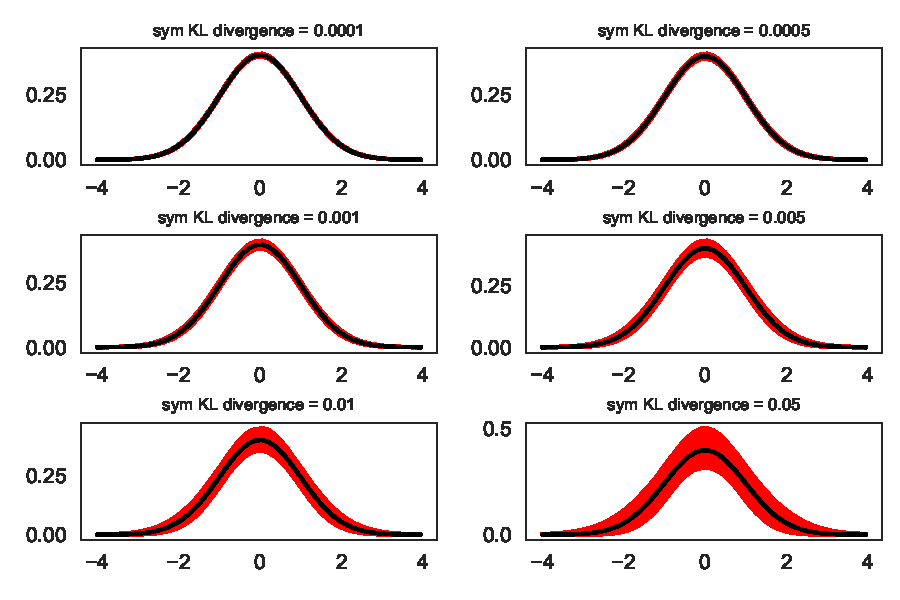
\includegraphics[scale=0.75,trim = 0cm .5cm 0cm 0cm]{images/KL_envelope}
\centering\caption{
An envelope of $\mathcal{N}(\epsilon_1, 1 + \epsilon_2)$ 1D Gaussian around an $\mathcal{N}(0,1)$ Gaussian for a family of $\epsilon_1$ and $\epsilon_2$ corresponding to various symmetric KL divergences.
}
\label{c2:KL_envelope}
\end{center}
\end{figure}
%%%%%%%%%%%%%%%%%%%%%%%%%%%%%%%%%%%%%%%%%%%%%%%%%%%%%%%%%%%%%%%%%%
%%%%%%%%%%%%%%%%%%%%%%%%%%%%%%%%%%%%%%%%%%%%%%%%%%%%%%%%%%%%%%%%%%%%%%%%%%%%%%
%%%%%%%%%%%%%%%%%%%%%%%%%%%%%%%%%%%%%%%%%%%%%%%%%%%%%%%%%%%%%%%%%%%%%%%%%%%%%%
\section{cgDNAmc$+$}\label{c2:sec6}
The cgDNA$+$ model predicts a Gaussian pdf (groundstate and stiffness matrix) for a given $\sq \and \Pc$.
This section briefly describes how to efficiently sample cgDNA$+$ Gaussian pdf and then use that ensemble of configurations to compute expectations of any function, particularly of various interesting physical observables such as persistence length and end-to-end distribution. 
Mitchell et al.~\cite{cgdnamc} developed a very efficient Monte-Carlo sampling method that allows generating a million samples in only a few minutes on a single processor for a given sequence of length 300 bps. 
The efficient sampling is due to the efficient Cholesky decomposition of the sparse banded stiffness matrix, $\K=LL^T$. 
The cgDNA$+$ Gaussian can be rewritten as; 
\begin{equation}
\rho(w; \sq, \mathcal{P}) 
= \frac{1}{\textit{Z}} e^{-\beta E(w)}
= \frac{1}{\textit{Z}} e^{-\beta y^Ty/2}
\label{c2:eq_mc}
\end{equation}
where $y=L^T(w-\hat{w})$ which can be easily sampled directly as product of independent uni-variate normal Gaussian distributions and the configuration in cgDNA$+$ variables can be obtained by solving $L^Tz=y$ and $w = z + \hat{w}$. 
More details can be found in ref.~\cite{cgdnamc}. 
Subsequently, using these configurations in cgDNA$+$ internal variables, the ensemble expectation of any function, $f(w)$ can be approximated as $\frac{1}{n}\sum_{i=1}^nf(w_i)$ where $n$ is the total number of configurations generated.

\subsection{Persistence length}\label{c2:s6sb1}
One of the interesting physical observables in the context of DNA is persistence length, which represents the inclination of a polymer to \enquote{persist} in a given direction.
It has been a popular and traditional measure to quantify the rigidity of DNA and is defined as the length scale over which correlations in the direction of tangent along a polymer centerline are lost~\cite{hagerman1988flexibility}. 
Mathematically, using the discrete version of Kratky-Porod Worm-Like Chain model~\cite{kratky1949}, the persistence length ($\ell_p$) for a linear chain of $N$ rigid bodies with the position $r_i|_{i=1,...,N}$ can be defined as; 
\begin{equation}
\langle t_i \cdot t_1  \rangle_{\text{WLC}} = e^{-i/\ell_p}
\label{c2:eq_persis}
\end{equation}
where $\langle \cdot  \rangle$ represents the ensemble average, $t_1$ and $t_i$ are the unit vectors for the base-pair index 1 and i along the DNA. 
$t_i$ can be defined as $t_i := (r_{i+1}-r_i)/b$ where rigid bodies are separated at length $b$ and $r_i$ is the position of the i$^\text{th}$ rigid body.

In the context of dsDNA (and other dsNAs), the definition of persistence length has been frequently used in the sequence-average sense, which has two crucial governing factors~\cite{trifonov1987dna}, stiffness and intrinsic shape, which can be deconvoluted as;
\begin{equation}
\frac{1}{\bar{\ell_p}} = \frac{1}{\bar{\ell_s}} + \frac{1}{\bar{\ell_d}}
\label{c2:eq_persis2}
\end{equation}
where $\bar{\ell_p}$, $\bar{\ell_s}$, and $\bar{\ell_d}$ are sequence-average apparent, static, and dynamic persistence length, respectively and  $\{ \hat{t}_i \cdot \hat{t}_1  \} = e^{-i/\bar{\ell_s}}$ where $\hat{t}_i$ is tangent at the i$^\text{th}$ position in the groundstate and $\{\cdot\}$ represents the average taken over an ensemble of sequences (thus, sequence-averaged persistence lengths).
Mitchell et al.~\cite{cgdnamc} generalized these definitions introducing sequence-dependent dynamic persistence length as 
\begin{equation}
\langle t_i \cdot t_1  \rangle = \{ \hat{t}_i \cdot \hat{t}_1  \} e^{-i/\ell_d}
\label{c2:eq_persis3}
\end{equation}
where $\{ \hat{t}_i \cdot \hat{t}_1  \}=e^{-i/\ell_s}$ is only evaluated at the groundstate of a given sequence, thus resulting in sequence-dependent $\ell_s$ and $\ell_d$.

cgDNAmc$+$ efficiently code this using just inter-coordinates.
Monte Carlo code samples a configuration, $w \in \R^{24N-18}$ as described in \cref{c2:eq7} and from $w$ extracts inter coordinates, \textit{y} and subsequently, the base-pair frames with orientation and position for i$^\text{th}$ base-pair frame given as $R_i \in SO(3)$ and $r_i$ (refer to \cref{c2:s2sb2} for details).
This work further simplifies the computations by approximating $t_i$ as base-pair normal (third column of $R_i$).
A detailed discussion of the various possible definitions of $t_i$ and their implications can be found in the original cgDNAmc article~\cite{cgdnamc}.
Now, $ t_i \cdot t_1 $ can be written as $(R_i^TR_1)_{33}$ and is computationally obtained as the inner-product of third column of $R_i$ and third column of $R_1$. 
The corresponding ensemble average can be computed as $\langle t_i \cdot t_1  \rangle = \frac{1}{n} \sum_i^n t_i \cdot t_1$ where $n$ is typically chosen as $10^5$ which provides sufficiently converged statistics~\cite{patelithesis}.
Lastly, $\ell_p$ and $\ell_d$ can be computed as the -1/slope of the linear fit, $\{ i,log(\langle t_i \cdot t_1  \rangle)\}|i=1,...,N$ and $\{i,log(\langle t_i \cdot t_1  \rangle) - log(\langle \hat{t}_i \cdot \hat{t}_1 \rangle )\}|_{i=1,...,N}$, respectively, where $N$ is the number of the base-pairs. 
Note that, in this work, the reference terminal base-pairs (i.e., $i=1$ and $i=N$) have been chosen away from the ends to avoid any end effects (i.e., six base-pairs from both sides have been dropped in the computation of persistence length).